\documentclass[10pt]{article}
\usepackage{CJKutf8}
\usepackage{amssymb}
\usepackage{amsthm}
\usepackage{mathtools}
\usepackage{amsmath}
\usepackage{amsfonts}
\usepackage{enumitem}
\usepackage[a4paper, left=2.5cm, right=2.5cm, top=1.25cm, bottom=1.25cm]{geometry}
\usepackage{multicol}
\usepackage{tikz-cd}
\usepackage{array}
\usepackage{makecell}
\usepackage{tabularx}
\setlength{\columnsep}{0.75cm}

\newtheorem{exercise}{Exercise}

\setlength{\parindent}{0cm}
\setlength{\parskip}{1em}

\DeclarePairedDelimiter\abs{\lvert}{\rvert}
\newcommand*{\qedfill}{\hfill\ensuremath{\blacksquare}}

\title{Sayako's Scratchpad}
\author{Sayako Hoshimiya}
\begin{document}
\begin{CJK*}{UTF8}{gbsn}
\maketitle
\renewcommand{\setminus}{\mathbin{\backslash}}
\def \setminus {\mathbin{\backslash}}
\textbf{Munkres Topology Problem 17.19.}
\newcommand{\Bd}{\text{Bd}\,}
\newcommand{\Int}{\text{Int}\,}
Let $A$ be a open subset of a topological space $X$. With $\Bd A$ denoting the boundary of $A$, as in the problem defined as the subset $\Bd A=A\cap X-A$. It is easy to see that $\overline{X-A}=X-\Int A$ (because $\Int A$ is the largest open set contained in $A$, and $X-\Int A$ is the smallest closed set containing $X-A$), so that we have
$$
\Bd A=\overline{A}\cap(X-\Int A)=\overline{A}-\Int A.
$$

The problem is solved by repeated use of the above equation.

\begin{enumerate}[label=(\alph*)]
\item With the above description of $\Bd A$, it is clear that $\Int A$ is disjoint with $\Bd A$. Furthermore, it follows, from the inclusion $\Int A\subset\overline{A}$, that $\overline{A}=\Int A\cup\Bd A$.

\item It is true that
\begin{align*}
A\text{ is both open and closed}&\iff A=\Int A=\overline{A}\\
&\iff\overline{A}\subset\Int A\\
&\iff\Bd A=\emptyset.
\end{align*}

\item It is true that
$$
U\text{ is open}\iff\Int U = U\iff\Bd U=\overline{U}-U,
$$
where the last implication follows from the fact that $U$ and $\Int U$ are subsets of $\overline{U}$.

\item If $U$ is open, $U=\Int U\subset\Int\overline{U}$ is true, but the reverse inclusion does not necessarily apply. We say, for example, $U=\mathbb{R}\setminus\{0\}$ gets $\Int\overline{U}=\mathbb{R}$.
\end{enumerate}

\newpage
\textbf{Exercise 7.16.} Suppose $\{f_n\}$ is an equicontinuous sequence of functions on a compact set $K$, and $\{f_n\}$ converges pointwise on $K$. Prove that $\{f_n\}$ converges uniformly on $K$.
\begin{proof}
For given $\varepsilon$, choose $\delta$ such that $\abs{x-y}<\delta$ implies $\abs{f_n(x)-f_n(y)}<\frac{\varepsilon}{3}$ where $n=1,2,\dots$ (this is possible since $\{f_n\}$ is equicontinuous). Define a set $S=\{B_\delta(x)\,\big|x\in K\}$, then it forms an open cover of $K$. By the compactness of $K$, there exists a finite subcover $\{B_\delta(x_1),B_\delta(x_2),\dots,B_\delta(x_k)\}$. Now choose $N_i\in\mathbb{N}$ for each $x_i$ such that $m,n>N_i$ implies $\abs{f_m(x_i)-f_n(x_i)}<\frac{\varepsilon}{3}$ (this is possible since $\{f_n\}$ converges pointwise, which suggests that each $\{f_n(x)\}_{n=1}^\infty$ is a Cauchy sequence). For each $x\in K$, choose $x_i$ such that $x\in B_\delta(x_i)$, then if $m,n>\max_i N_i$,
$$
\abs{f_m(x)-f_n(x)}\leq\abs{f_m(x)-f_m(x_j)}+\abs{f_m(x_j)-f_n(x_j)}+\abs{f_n(x_j)-f_n(x)}<\frac{\varepsilon}{3}+\frac{\varepsilon}{3}+\frac{\varepsilon}{3}=\varepsilon.
$$
\end{proof}

\textbf{Exercise 7.18.} Let $\{f_n\}$ be a uniformly bounded sequence of functions which are Riemann-integrable on $[a,b]$, and put
$$
F_n(x)=\int_a^xf_n(t)\operatorname{d}t\quad(a\leq x\leq b).
$$
Prove that there exists a subsequence $\{F_{n_k}\}$ which converges uniformly on $[a,b]$.
\begin{proof}
Since $\{f_n\}$ is uniformly bounded, there exists $M$ such that $\abs{f_n(x)}<M$ for all $x\in[a,b]$ and $n=1,2,\dots$. It is clear that
$$
\abs{F_n(x)}=\left|\int_a^xf_n(t)\operatorname{d}t\right|\leq\int_a^x\abs{f_n(t)}\operatorname{d}t\leq\int_a^xM\operatorname{d}t\leq\int_a^bM\operatorname{d}t=M(a-b),
$$
which suggests that $F_n(x)$ is uniformly bounded. Now for any $\varepsilon$, there exists $\delta=\frac{\varepsilon}{M}$, such that for any $x,y\in[a,b]$, $\left|x-y\right|<\delta$ implies
$$
\abs{F_n(x)-F_n(y)}=\left|\int_a^xf_n(t)\operatorname{d}t-\int_a^yf_n(t)\operatorname{d}t\right|=\left|\int_y^xf_n(t)\operatorname{d}t\right|\leq\left|\int_y^xM\operatorname{d}t\right|=\abs{x-y}M<\varepsilon,
$$
and this means that function family $\{F_n(x)\}$ is equicontinuous.
The functions are clearly defined on a compact set, then by Arzel\`a-Ascoli Theorem (Theorem 7.25(b)), there exists a uniformly convergent subsequence of $\{F_n\}$.
\end{proof}

\newpage
\textbf{第一题}
\begin{enumerate}
\item 试叙述$\mathbb{R}^n$中的一个集合为连通集的定义:

拓扑空间$\mathbb{R}^n$的子集$A$被称为连通集当且仅当$A$不能被分割成两个在$A$的子空间拓扑上的非空不交开子集。

\item 试证明$\mathbb{R}^n$中的集合$D$不是连通集当且仅当存在连续映射$f:D\to\{0,1\}$使得$f$为一满射:

首先证明$(\impliedby)$方向。对$D$使用$X=\mathbb{R}^n$的通常拓扑在$D$上的子空间拓扑,对$\{0,1\}$使用离散拓扑。因为$f$为连续映射,开集$\{0\}$的原像是开集,又因$f$是满射,$f^{-1}(\{0\})\neq\emptyset$;同样的性质对$\{1\}$也成立。由于$f$是映射,$\lnot\exists x\in D.\, f(x)=0\land f(x)=1$,换句话说,$f^{-1}(\{0\})\cap f^{-1}(\{1\})=\emptyset$。$D$的子集$f^{-1}(\{0\})$和$f^{-1}(\{1\})$分割集合$D$、是开集、非空、不交,由此说明$D$不是一个连通集。

再证明$(\implies)$方向。使用的拓扑与前文相同。$D$不是连通集意味着存在两个非空不交开集$A,B\subset D$使得$D=A\cup B$。定义映射
$$
f(x)=\begin{cases}
0\quad x\in A\\
1\quad x\in B
\end{cases},
$$
明显$\text{Dom}(f)=D$;由于$A,B\neq\emptyset$,$\text{Range}(f)=\{0,1\}$,即$f$是满射;所有开集的原像
\begin{align*}
f^{-1}(\{0\})&=A\\
f^{-1}(\{1\})&=B\\
f^{-1}(\emptyset)&=\emptyset\\
f^{-1}(\{0,1\})&=D
\end{align*}
均为开集,即$f$连续,$f$即为所需函数。\qed

\item 设$E\subset\mathbb{R}^n$为一连通集,试证明其闭包$\overline{E}$也是连通集:

证明此命题的逆否命题,即证明若$\overline{E}$不是连通集,则$E$不是连通集。根据前提,存在连通不交开集(相对于$\overline{E}$的子空间拓扑)$A,B\subset\overline{E}$使得$\overline{E}=A\cup B$。对于任意$x\in A$,$x\in E$或$x$是$E$的极限点。记$S_A=\{x\in E\,\big|\,x\in A\}$,则$S_A\neq\emptyset$,因为若$x\in A$是$E$的极限点,开集$A$包括$x$,则存在$y\in A$使得$y\in E$;同理可构造$S_B$。此时记$S_A=A\cap E$,$S_B=B\cap E$,即$S_A,S_B$为$E$的子空间拓扑中的开集;根据构造,$S_A,S_B$不交且非空,由此证明了$E$不是连通集。\qed

\end{enumerate}

\textbf{第四题}

设$f:\mathbb{R}^2\to\mathbb{R}$为一连续可微函数。试证存在连续可微的单射$\phi:(0,1)\to\mathbb{R}^2$使得$f\circ\phi$为$(0,1)$上的常值函数。

\textbf{第五题}

给定$\mathbb{R}^n$中的有界开集$\Omega$及其紧致子集$D$。设$f:\Omega\to\mathbb{R}^n$为一连续可微映射,$f$在$D$上的限制为一单射并且对任意$x\in D$有$\det(f'(x))\neq0$。
\begin{enumerate}
\item 证明$d(D,\partial\Omega)>0$:

首先证明$\Omega$与$\partial\Omega$不交,即与$D$不交。记拓扑空间$\mathbb{R}^n=X$根据边界的定义,$\partial\Omega=\overline{\Omega}\cap\overline{(X\setminus\Omega)}$,即$\partial\Omega\subset\overline{(X\setminus\Omega)}$。因$\Omega$是开集,其补集$X\setminus\Omega$为闭集,根据闭包定义,$\overline{X\setminus\Omega}=X\setminus\Omega$。因此,$\partial\Omega\subset X\setminus\Omega$,即$\partial\Omega\cap\Omega=\emptyset$。

假设$d(D,\partial\Omega)=0$,即$\inf\{d(x,y)\,\big|\,x\in D,y\in\partial\Omega\}=0$,即对于任意$\varepsilon>0$,存在$x\in D,\,y\in\partial\Omega$使得$\abs{x-y}<\varepsilon$,其中$y\notin D$。定义集合$S_{\frac{1}{n}}=\{x\in D\,\big|\,d(x,\partial\Omega)>\frac{1}{n}\}$,根据先前论证,若$\frac{1}{m}<\frac{1}{n}$,$S_{\frac{1}{n}}\subset S_{\frac{1}{m}}$,且$\bigcup_{n\in\mathbb{Z}^+}S_{\frac{1}{n}}=D$。此时集合族$S=\{S_{\frac{1}{n}}\}_{n\in\mathbb{Z}^+}$构成集合$D$的一个开覆盖,但这个开覆盖没有有限子覆盖,因为对于$S$的任何有限子集$S'=\{S_{\frac{1}{n_k}}\}_{k=1}^N$,都可找到一个$x\in D$使得$d(x,\partial\Omega)<\min\{\frac{1}{n_k}\}_{k=1}^N$,即$x\notin\bigcup_{k=1}^N S_{\frac{1}{n_k}}$,则$S‘$不是$D$的有限子覆盖,由此与前提$D$的紧致性矛盾。\qed
\end{enumerate}

\newpage
\textbf{Theorem (Lagrange's Mean Value Theorem).} For any real function $f:I\to\mathbb{R}$ that is continuous on $[a,b]\subset I$ and differentiable on $(a,b)$, there exists $\xi\in(a,b)$ such that
$$
f'(\xi)=\frac{f(b)-f(a)}{b-a}.
$$

\textbf{Question.} For any function $f$ satisfying the premises of the Lagrange's Mean Value Theorem, namely continuous on $[a,b]$ and differentiable on $(a,b)$, show that if $f(a)=f(b)=0$, then there exists $\xi\in(a,b)$ such that
$$
f'(\xi)+f(\xi)=0.
$$

\vspace{6em}
\textbf{Solution.} Apply the Lagrange's Mean Value Theorem on function $f(x)e^x$, then there exists $\xi\in(a,b)$ such that
$$
f'(\xi)e^\xi+f(\xi)e^\xi=\frac{f(b)e^b-f(a)e^a}{b-a}.
$$
Since $f(a)=f(b)=0$,
$$
f'(\xi)e^\xi+f(\xi)e^\xi=0.
$$
Since $e^\xi\neq0$ for all real $\xi$,
$$
f'(\xi)+f(\xi)=0.
$$\qed

\newpage
\textbf{Question (Integrability and Integral of Thomae Function).} Define function $f:[0,1]\to\mathbb{R}$ as
\begin{align*}
f(x)=\begin{dcases}
\frac{1}{q}&x=\frac{p}{q},\,p,q\in\mathbb{N},\,(p,q)=1\\
0&x\in\mathbb{R}\setminus\mathbb{Q}
\end{dcases},
\end{align*}
decide whether $f$ is Darboux-integrable; if so, prove it so and calculate its integral; if not, prove it otherwise.

\textbf{Solution.} It is obvious that $L(f,\Delta)=0$ for any partition $\Delta$, since any closed interval contains both rational and irrational number, thus $\displaystyle\sup_\Delta L(f,\Delta)=0$. It is also clear that for any $\Delta$, $U(f,\Delta)>0$, again, since rational numbers exists in any closed interval.

For $\varepsilon>0$, choose $m$ such that $\frac{1}{m}<\frac{\varepsilon}{2}$, then for any partition $\Delta_1=\{x_0,x_1,\dots,x_k\}$ such that each rational number $\frac{1}{n}$ where $n<m$ is contained in exactly one subinterval, i.e. not on the endpoint of any subinterval, each subinterval $[x_{i-1},x_i]$ of partition containing $\frac{1}{n}$ where $n\geq m$ and no rational number with denominator less than $m$ will have a supremum less than $\frac{1}{m}$. Denote the set of indices of the right endpoints of these subintervals as $S_1$, and sum them up,
$$
\sum_{i\in S_1}\sup f(x)\cdot(x_i-x_{x-1})<\sum_{i\in S_1}\frac{1}{m}\cdot(x_i-x_{x-1})<\sum_{i=1}^k\frac{1}{m}\cdot(x_i-x_{x-1})=\frac{1}{m}=\frac{\varepsilon}{2}.
$$

For those subintervals that contains the rest of the rational numbers, i.e. those with denominator less than $m$, choose partition $\Delta_2$ such that the length (right endpoint minus left endpoint) of each subinterval containing these rational numbers is less than $\displaystyle l=\frac{\varepsilon}{2\cdot\frac{(m-1)^2}{2}}$. Denote the set of indices of the right endpoints of these subintervals as $S_2$, and observe the cardinality of $S_2$. List possible fractions $\frac{p}{q}$ as
$$
\frac{1}{1},\frac{1}{2},\frac{2}{2},\cdots,\frac{1}{m-1},\frac{2}{m-1},\cdots,\frac{m-1}{m-1},
$$
it is clear there are duplication, and thus $|S_2|\leq\frac{(m-1)^2}{2}$. Sum them up,
$$
\sum_{i\in S_2}\sup f(x)\cdot(x_i-x_{x-1})<\sum_{i\in S_2}\sup f(x)\cdot l\leq\sum_{i\in S_2}l=|S_2|\cdot l\leq\frac{(m-1)^2}{2}\cdot\frac{\varepsilon}{2\cdot\frac{(m-1)^2}{2}}=\frac{\varepsilon}{2}.
$$

Now find the common partition of the two previously mentioned partitions, i.e. $\Delta=\Delta_1\cup\Delta_2$, then
$$
U(f,\Delta)=\sum_{i\in S_1}\sup f(x)\cdot(x_i-x_{x-1})+\sum_{i\in S_2}\sup f(x)\cdot(x_i-x_{x-1})<\varepsilon.
$$
And this shows that $\displaystyle\inf_\Delta U(f,\Delta)=0$, which decides that $f$ is Darboux-integrable with integral $0$.

\newpage
\textbf{Lemma.} For matrix $A=(a_{i,j})_{n\times n}$, $B=(b_{i,j})_{n\times n}$, $AB=c_{i,j}$ satisfying properties
\begin{equation}
a_{i,j}=0\quad\text{for}\quad j<i+r\quad(r\geq1)
\end{equation}
and
\begin{equation}
\label{2}
b_{i,j}=0\quad\text{for}\quad j<i+1,
\end{equation}
it is guaranteed that for $j<i+r+1$
$$
c_{i,j}=0.
$$
\begin{proof}
For $j<i+r$, by (1) we have
\begin{equation}
\label{3}
\sum_{k=1}^na_{i,k}b_{k,j}=0\cdot b_{k,j}=0.
\end{equation}

For $j=i+r$, perform case analysis on $k$. If $k<i+r$, by (1) we have
\begin{equation}
\label{4}
\sum_{k=1}^{i+r-1}a_{ik}b_{k,j}=0\cdot b_{k,j}=0.
\end{equation}

If $k\geq i+r$, then $j=i+r<i+r+1=k+1$, thus by (2) we have
\begin{equation}
\label{5}
\sum_{k=i+r}^{n}a_{ik}b_{k,j}=a_{i,k}\cdot0=0.
\end{equation}

Combine (4) and (5), we have for $j=i+r$, $c_{i,j}=0$.
Combine this with (3), we have for $j<i+r+1$, $c_{i,j}=0$, as desired.
\end{proof}

\textbf{Theorem.} For square strictly upper triangular matrix $S$, $(S^k)_{i,j}=0$ for $j<i+k$ ($1\geq k\geq n$).
\begin{proof}
Prove by induction on $k$. From the definition of strictly upper triangular matrix and the previous proven lemma, base case $k=1$ holds. For the induction case, the induction hypothesis is that $(S^k)_{i,j}=0$ for $j<i+k$. Write $S^{k+1}=S^k\cdot S$, which again satisfies the premises of the lemma, thus $(S^{k+1})_{i,j}=0$ for $j<i+k+1$
\end{proof}

\textbf{Corollary.} For $n\times n$ strictly upper triangular matrix $S$, $S^n=(0)_{n\times n}$.
\begin{proof}
By the previous theorem, $(S^n)_{i,j}=0$ for $j<i+n$, thus $(S^n)_{i,j}=0$ for all $1\geq i,j\geq n$.
\end{proof}

\newpage
\textbf{Question from Kristall.} Let $A$ be an $n\times n$ square matrix and suppose $x$ and $y$ are non-zero $n$-vectors satisfying $Ax = x$ and $Ay = \gamma y$, where $\gamma\neq1$. Show that $\{x, y\}$ is a linearly independent set in $\mathbb{R}^n$.

\textbf{Solution.} Suppose the contrary, i.e. $\{x,y\}$ is linearly dependent in $\mathbb{R}^n$, which is to say that there exists $\alpha_1,\alpha_2$ such that $$\alpha_1x+\alpha_2y=0.$$ Then by the property of the underlying field $\mathbb{R}$ of the vector space $\mathbb{R}^n$, $$y=-\frac{\alpha_1}{\alpha_2}x.$$ By the premise $Ay=\gamma y$, $$A\left(-\frac{\alpha_1}{\alpha_2}x\right)=\gamma\left(-\frac{\alpha_1}{\alpha_2}x\right).$$ By property of linear transformation, $$\left(-\frac{\alpha_1}{\alpha_2}\right)(Ax)=\left(-\frac{\alpha_1}{\alpha_2}\right)\gamma x.$$ By the cancellative property of $\mathbb{R}$, $$Ax=\gamma x,$$ which, together with the premise $\gamma\neq1$, contradicts the premise $Ax=x$, and this establishes the proposition.

\newpage
\textbf{Lemma.} For a sequence $\{a_n\}$, if $$\lim_{k\to\infty}\frac{1}{k}\sum_{n=1}^ka_n=A,$$ then $\displaystyle\lim_{n\to\infty}a_n=A$.

\textbf{Proof to Lemma.} By the definition of limit, the premise can be explicitly written as $$\forall\varepsilon>0.\,\exists K\in\mathbb{N}.\,\forall k>K.\,\left|\frac{1}{k}\sum_{n=1}^{k}a_n-A\right|<\varepsilon.$$ Expand the absolute value and move terms, we have $$kA-k\varepsilon<\sum_{n=1}^ka_n<kA+k\varepsilon;$$ since $k$ can be any number greater than $K$, the condition still holds for $k=k+1$, i.e. $$(k+1)A-(k+1)\varepsilon<\sum_{n=1}^{k+1}a_n<(k+1)A+(k+1)\varepsilon.$$ Subtracting the $k$ case from the $k+1$ case, we have $$A-\varepsilon<a_{k+1}<A+\varepsilon,$$ which in turn gives the desired conclusion, i.e. $|a_{k+1}-A|<\varepsilon$.\qed

\textbf{Lemma.} For continuously differentiable function $f:[a,b]\to\mathbb{R}$, there exists $\xi\in(a,b)$ such that $$\int_a^bf(x)\operatorname{d}x=f(\xi)(b-a).$$

\textbf{Proof to Lemma.} Apply Lagrange's Mean Value Theorem to the function $F(x)$ where $F'(x)=f(x)$, then the result is obvious.\qed

\textbf{Proposition.} For continuous function $f$ such that $\displaystyle\lim_{a\to\infty}I_a=A$ where $$I_a=\frac{1}{a}\int_0^af(x)\operatorname{d}x,$$ there exists a strictly monotonically increasing sequence $\{x_n\}$ such that $\displaystyle\lim_{n\to\infty}x_n=\infty$ and $\displaystyle\lim_{n\to\infty}f(x_n)=A$.

\textbf{Proof to Proposition.} Construct the sequence $\{x_n\}$ with following step. First, for $a\in\mathbb{N}$, write $$I_a=\frac{1}{a}\sum_{n=1}^a\int_{n-1}^nf(x)\operatorname{d}x.$$ Apply the previous lemma, we have that $$\lim_{n\to\infty}\int_{n-1}^nf(x)\operatorname{d}x=A.$$ The previous lemma gives rise to the existence of the desired sequence.\qed

\newpage
\textbf{Ben Andrews Lecture on Differential Geometry - Exercise 1.1.1}

\textbf{Exercise.} Define $\mathbb{C}P^n$ to be $(\mathbb{C}^{n+1}\setminus\{0\})/\sim$, where $x\sim y$ if and only if $x=\lambda y$ for some $\lambda\in\mathbb{C}\setminus\{0\}$. Find a differentiable atlas which makes $\mathbb{C}P^n$ a $2n$-dimensional smooth manifold.

\textbf{Solution.} Inspired by observing the case for the real projective plane $\mathbb{R}P^n$, we proceed with the following construction. First define the homeomorphisms $f_i$ from a subset of the complex projective hyperplane to the complex Euclidean space of dimension $n$ as \begin{align*}f_i:U_i=\{x\,\big|\,x\in\mathbb{C}P^n,x_i\neq0\}\subset\mathbb{C}P^n&\to\mathbb{C}^n\\\lbrack x\rbrack&\mapsto\frac{1}{x_i}\langle x_1,\dots,\widehat{x_i},\dots,x_{n+1}\rangle,\end{align*} which are well-defined since under a change of representative, i.e. for any $y=\lambda x$, $$\frac{1}{y_i}\cdot y=\frac{1}{\lambda x_i}\cdot\lambda x=\frac{1}{x_i}\cdot x.$$

We claim that $\{(U_i,\mathbb{1}^{n\to2n}_{\mathbb{C}\to\mathbb{R}}\circ f_i)\}_{i=1,\dots,n+1}$ is an atlas contained in the differentiable structure of $\mathbb{C}P^n$; it's easy to verify that is does cover $\mathbb{C}P^n$, and now we will verify other properties.

For any $i$, we prove the injectivity of $f_i$ as follows. A complex vector $\tilde{x}\in\mathbb{C}^n$ to differ from $\tilde{y}\in\mathbb{C}^n$, it must differ therefrom in at least one component; assume those components are $\tilde{x}_j\neq\tilde{y}_j$, then for any representative $x=\lambda_1\langle\tilde{x}_1,\dots,1,\dots,\tilde{x}_{n+1}\rangle$ (the $1$ is at the $i$-th position) of $f_i^{-1}(\tilde{x})$ and any representative $y=\lambda_2\langle1,\tilde{y}_1,\dots,\tilde{y}_{n+1}\rangle$ of $f_i^{-1}(y')$, for any $\lambda\in\mathbb{C}\setminus\{0\}$, in order for the $j$-th component ($j=1,\dots,i-1,i+1,\dots,n$) of $x$ and $y$ to agree, one must have $\lambda=\frac{\lambda_1x_i}{\lambda_2y_i}$, and for the $i$-th component to agree, $\lambda=\frac{\lambda_1}{\lambda_2}$, and thus $x_i=y_i$, which contradicts the premise that $x_i\neq y_i$ and disprove the existence of such $\lambda$ and in turn gives $f_i^{-1}(\tilde{x})\neq f_i^{-1}(\tilde{y})$ and thus the injectivity.

Surjectivity is trivial since for any $x=\langle x_1,\dots,x_n\rangle\in\mathbb{C}^n$, we have $f_i(\lbrack\langle x_1,\dots,1,\dots,x_n\rangle\rbrack)=x$.

For continuity, we immediately notice that the function $$g_i:\langle x_1,\dots,x_i,\dots,x_{n+1}\rangle\mapsto\frac{1}{x_i}\langle x_1,\dots,\widehat{x_i},\dots,x_{n+1}\rangle$$ is continuous since $x_i\neq0$. But $f_i$ is just the quotient induced map $\overline{g}_i$ such that $\overline{g}_i\circ\pi=g_i$ and is continuous since $\pi$ and $g_i$ are both continuous. For inverse continuity, we observe that $f^{-1}_i=\pi\circ h_i$ where $$h_i:\langle x_1,\dots,x_n\rangle\mapsto\langle x_1,\dots,x_{i-1},1,x_{i},\dots,x_n\rangle$$ which is continuous when the codomain is $\{x\in\mathbb{C}^n\,\big|\,x_i=1\}$ with its subspace topology; and this proves the inverse continuity. Since $\mathbb{1}^{n\to2n}_{\mathbb{C}\to\mathbb{R}}$ is a homeomorphism, we have thus shown that $\mathbb{1}^{n\to2n}_{\mathbb{C}\to\mathbb{R}}\circ f_i$ are homeomorphisms.

To prove that the aforementioned atlas is a part of the differentiable structure on $\mathbb{C}P^n$, we need to show the transition maps \begin{align*}\varphi^i_j=(\mathbb{1}^{n\to2n}_{\mathbb{C}\to\mathbb{R}}\circ f_j)\circ(f^{-1}_i\circ\mathbb{1}^{2n\to n}_{\mathbb{R}\to\mathbb{C}})\end{align*} are smooth. By basic complex analysis, the components of this function is $$\frac{x_kx_j+x_{k+1}x_{j+1}}{x_j^2+x_{j+1}^2},\frac{x_{k+1}x_j-x_kx_{j+1}}{x_j^2+x_{j+1}^2}$$ for $k=1,\dots,n$; there are two groups of $1,0$, one of which (the one at position $2j$ and $2j+1$) is to be omitted; and this leaves us with exactly $2n$ components. These components are all smooth since $(x_j,x_{j+1})\neq(0,0)$; we have proven the smoothness of transition maps, and thus the atlas being contained in the differentiable structure.\qed

\newpage
\textbf{UIUC Math 525 Spring 2018 Homework 1}

\textbf{Problem 1.} Let $X$ and $Y$ be topological spaces. Suppose $A_1$ and $A_2$ are closed subsets of $X$ such that $X=A_1\cap A_2$. If $f_i:A_i\to Y$ are continuous functions that agree on $A_1\cap A_2$, show that the function $$f:X\to Y,\quad f(x)=\begin{cases}f_1(x)\quad\text{if }x\in A_1\\f_2(x)\quad\text{if }x\in A_2\end{cases}$$ is continuous.

\textbf{Solution.} [This is sometimes referred to as the pasting lemma, and it's of theoretical significance in the studies of algebraic topology.] For closed set $U$ in $Y$, its preimages $f_1^{-1}(U)$ and $f_2^{-1}(U)$ are closed respectively in $A_1$ and $A_2$ since these functions are continuous; and they are closed in $X$ since $A_1$ and $A_2$ are closed in $X$. By basic set theory, $f^{-1}(U)=f_1^{-1}(U)\cup f_2^{-1}(U)$, and the union of two closed sets are closed, thus the function $f$ is continuous.

\textbf{Problem 2.} Show that a space $X$ is contractible iff every map $f:X\to Y$, for arbitrary $Y$, is nullhomotopic. Similarly, show $X$ is contractible iff every map $f:Y\to X$ is nullhomotopic.

\textbf{Solution.} $(\impliedby)$ Take the map $f:X\to X$; by premise it's nullhomotopic, i.e. there exists a homotopy $f_t(x)$ from $\mathbb{1}_X$ to constant map $x\mapsto x_0$; this implies precisely that $X$ is contractible. $(\implies)$ If $X$ is contractible, then there exists a homotopy between the identity map $\mathbb{1}_X$ and a constant map $x\mapsto x_0$; denote it $A_t(x)$. For any function $f:X\to Y$, define the homotopy $B_t(x)=f(A_t(x))$, then it is a homotopy between $f$ and the constant map $x\mapsto f(x_0)$. The other statement can be proven similarly.

\textbf{Problem 3.} Show that $f:X\to Y$ is a homotopy equivalence if there exist maps $g,h:Y\to X$ such that $f\circ g\simeq\mathbb{1}_Y$ and $h\circ f\simeq\mathbb{1}_X$. More generally, show that $f:X\to Y$ is a homotopy equivalence if there exist $g,h:Y\to X$ such that $f\circ g$ and $h\circ f$ are homotopy equivalences.

\textbf{Solution.} Define function $\phi=h\circ f\circ g$. Denote the homotopy $f\circ g\simeq\mathbb{1}_Y$ as $A_t(y)$ and $h\circ f\simeq\mathbb{1}_X$ as $B_t(x)$. For the latter statement, if there exists $\alpha:Y\to Y$ and $\beta:X\to X$ such that $\alpha\circ f\circ g\simeq\mathbb{1}_Y\simeq f\circ g\circ\alpha$ and $\beta\circ h\circ f\simeq\mathbb{1}_X\simeq h\circ f\circ\beta$, then $g\circ\alpha$ would be the new $g$ and $\beta\circ h$ the new $h$ in the previous statement, thus the latter statement is a corollary.

\textbf{Problem 4.} Show that the number of path components is a homotopy invariant.

\textbf{Solution.} Let $X$ and $Y$ be two topological spaces, and $f:X\to Y$ and $g:Y\to X$ two maps such that $f\circ g\simeq\mathbb{1}_X$ with homotopy $A_t(x)$ and $g\circ f\simeq\mathbb{1}_Y$ with $B_t(y)$. We now define the bijection between the path components of $X$ and of $Y$ by $h([x])=[f(x)]$; this is well-defined since under a change of representative $x\sim y$, i.e. a path $p$ from $x$ to $y$, for we have path $f\circ p$ in $Y$ connecting $f(x)$ and $f(y)$. We claim that $h$ is injective, for if $h([x])=h([y])$, that is, $f(x)$ is connected with $f(y)$ by path $q$, then $$(t\mapsto B_{(1-t)}(x))*(g\circ q)*(t\mapsto B_t(y))$$ is a path from $x$ through $(g\circ f)(x)$ then $(g\circ f)(y)$ to $y$ thus asserting $x\sim y$ thus $[x]=[y]$. We then claim $h$ is surjective. For a path component $[z]$ in $Y$, that $[z]=[f(g(z))]$ is proven by constructing the path $r(t)=A_t(z)$, and $[z]=h([g(z)])=[f(g(z))]$, thus the surjectivity.

\textbf{Problem 5.} Show that for a space $X$, the following three conditions are equivalent:
\begin{enumerate}[label=(\alph*),nosep]
\item Every map $\mathbb{S}^1\to X$ [is] homotopic to a constant map, with image a point.
\item Every map $\mathbb{S}^1\to X$ extends to a map $\mathbb{D}^2\to X$.
\item $\pi_1(X,x_0)=0$ for all $x_0\in X$.
\end{enumerate}
Deduce that a space $X$ is simply connected iff all maps $\mathbb{S}^1\to X$ are homotopic.

\textbf{Solution.} (a)$\implies$(b) Parameterize the $1$-sphere by angle $\theta$. Denote the homotopy between the map and constant map as $f_t(\theta)$. This map extends to the map \begin{align*}g:\mathbb{D}^2&\to X\\(r,\theta)&\mapsto f_{1-t}(\theta),\end{align*} as desired. (b)$\implies$(c) For any given loop $f$ in $X$ starting and ending at $x_0$, we prove that it is path homotopic to the constant map to $x_0$. Define $g:\mathbb{S}^1\to X$ by $\theta\to f(\frac{\theta}{2\pi})$. Then by (b) there exists map $h:\mathbb{D}^2\to X$ that extends continuously the map $g$. Define the coordinate transformation map \begin{align*}\phi:\mathbb{R}^2&\to\mathbb{D}^2\\(x,y)&\mapsto\left(\sqrt{x^2+y^2},\begin{dcases}\lim_{x'\to x^+}\arctan\left(\frac{y}{x'}\right)\text{ if }y\geq0\\\lim_{x'\to x^-}\arctan\left(\frac{y}{x'}\right)\text{ if }y<0\end{dcases}\right).\end{align*} Define a map that shrinks the circle to a point at $(1,0)$ continuously as \begin{align*}\psi:[0,1]\times\mathbb{S}^1&\to\mathbb{R}^2\\(t,\theta)&\mapsto((1-t)\cos\theta+t,(1-t)\sin\theta).\end{align*} Now define the desired homotopy $A_t(s)=h(\phi(\psi_t(2\pi s)))$. (c)$\implies$(a) Trivial by definition.\qed

\textbf{Problem 6.} Given a space $X$, a path connected subspace $A$, and a point $x_0\in A$, show that the map $\pi_1(A,x_0)\to\pi_1(X,x_0)$ induced by the inclusion $A\hookrightarrow X$ is surjective iff every path in $X$ with endpoints in $A$ is homotopic, relative to its endpoints, to a path in $A$.

\textbf{Solution.} $(\impliedby)$ Denote the map as $f$. For $[x]\in\pi_1(X,x_0)$, it is a path in $X$ with endpoints in $A$, so it is path homotopic to a path $a$ in $A$, and since $x$ is a loop, so is $a$, thus $[a]\in\pi_1(A,x_0)$, and by the aforementioned path homotopy, $[a]=[x]$, so that $f([a])=[a]=[x]\in\pi_1(X,x_0)$. $(\implies)$ Suppose there exists a path $p$ in $X$ with endpoints $a,b$ in $A$ that is not path homotopic to any path in $A$. Since $A$ is path connected, there exists a path $q$ from $b$ to $a$ in $A$. We claim that $[p*q]\in\pi_1(X,x_0)$ and $[p*q]\notin\pi_1(A,x_0)$, i.e. $f$ defined above is not surjective. The former statement is trivial; the latter statement is true, for if not, that is $p*q\simeq a$ for some path $a$ in $A$, then $p\simeq a*\overline{q}$ would be a path in $A$, contradicting the premise.\qed

\newpage
\textbf{New Mathematics, Gaokao, and the School of Bourbaki}

\textbf{1 (Set Theory and Function).} \begin{itemize}
\item $f(f^{-1}(Y))\subset Y$ (equality when $f$ is surjective)
\item $X\subset f^{-1}(f(X))$ (equality when $f$ is injective)
\end{itemize}

\textbf{2 (Set Theory and Basic Topology).} For $f:A\times B\to C$, define $f_{1,a_0}(b)=f(a_0,b)$ and $f_{2,b_0}(a)=f(a,b_0)$. For $V\subset C$ and $(a_0,b_0)\in V$,
\begin{itemize}
\item $(\checkmark)$ $\{(a_0,b)\,|\,b\in f_{1,a_0}^{-1}(V)\}\cup\{(a,b_0)\,|\,a\in f_{2,b_0}^{-1}(V)\}\subset f^{-1}(V)$
\item $(\times)$ $\{(a_0,b)\,|\,b\in f_{1,a_0}^{-1}(V)\}\cup\{(a,b_0)\,|\,a\in f_{2,b_0}^{-1}(V)\}\underset{\text{open}}{\subset}A\times B$
\item $(\checkmark)$ $f_{2,b_0}^{-1}(V)\times f_{1,a_0}^{-1}(V)\underset{\text{open}}{\subset}A\times B$
\item $(\times)$ $f_{2,b_0}^{-1}(V)\times f_{1,a_0}^{-1}(V)\subset f^{-1}(V)$
\end{itemize}

\textbf{3 (Trigonometry and Calculus).} Every map $\mathbb{S}^1\to X$ extends to a map $\mathbb{D}^2\to X$ $\implies$ $\pi_1(X,x_0)=0$ for all $x_0\in X$. [The concept of fundamental group of a topological space can be replaced by something more elementary, or the basic idea of homotopy can be introduce on the go.]
\begin{align*}\phi:\mathbb{R}^2&\to\mathbb{D}^2\\(x,y)&\mapsto\left(\sqrt{x^2+y^2},\begin{dcases}\lim_{x'\to x^+}\arctan\left(\frac{y}{x'}\right)\text{ if }y\geq0\\\lim_{x'\to x^-}\arctan\left(\frac{y}{x'}\right)\text{ if }y<0\end{dcases}\right).\end{align*}
\begin{align*}\psi:[0,1]\times\mathbb{S}^1&\to\mathbb{R}^2\\(t,\theta)&\mapsto((1-t)\cos\theta+t,(1-t)\sin\theta).\end{align*}
$$A_t(s)=h(\phi(\psi_t(2\pi s)))$$

\textbf{4 (Trigonometry or Calculus).} Determine the area of the intersection of a unit circle and the area swiped by a vertical line from $x=-1$ to $x=a$ where $-1\leq a\leq 1$, i.e. determine the area surrounded by the circle and the chord.

\textbf{5 (Algebra).} A certain grassroots mathematician claims that $0$ can be a divider. Show them that there exists not any field with distinct additive and multiplicative identity that includes the inverse of the additive identity.

https://www.zhihu.com/question/317892880/answer/638183808

\textbf{6 (Sequence and Series).} $\displaystyle\sum_{k=0}^\infty \frac{k}{2^k}$

\newpage
\textbf{7 (Calculus).}
\begin{center}
	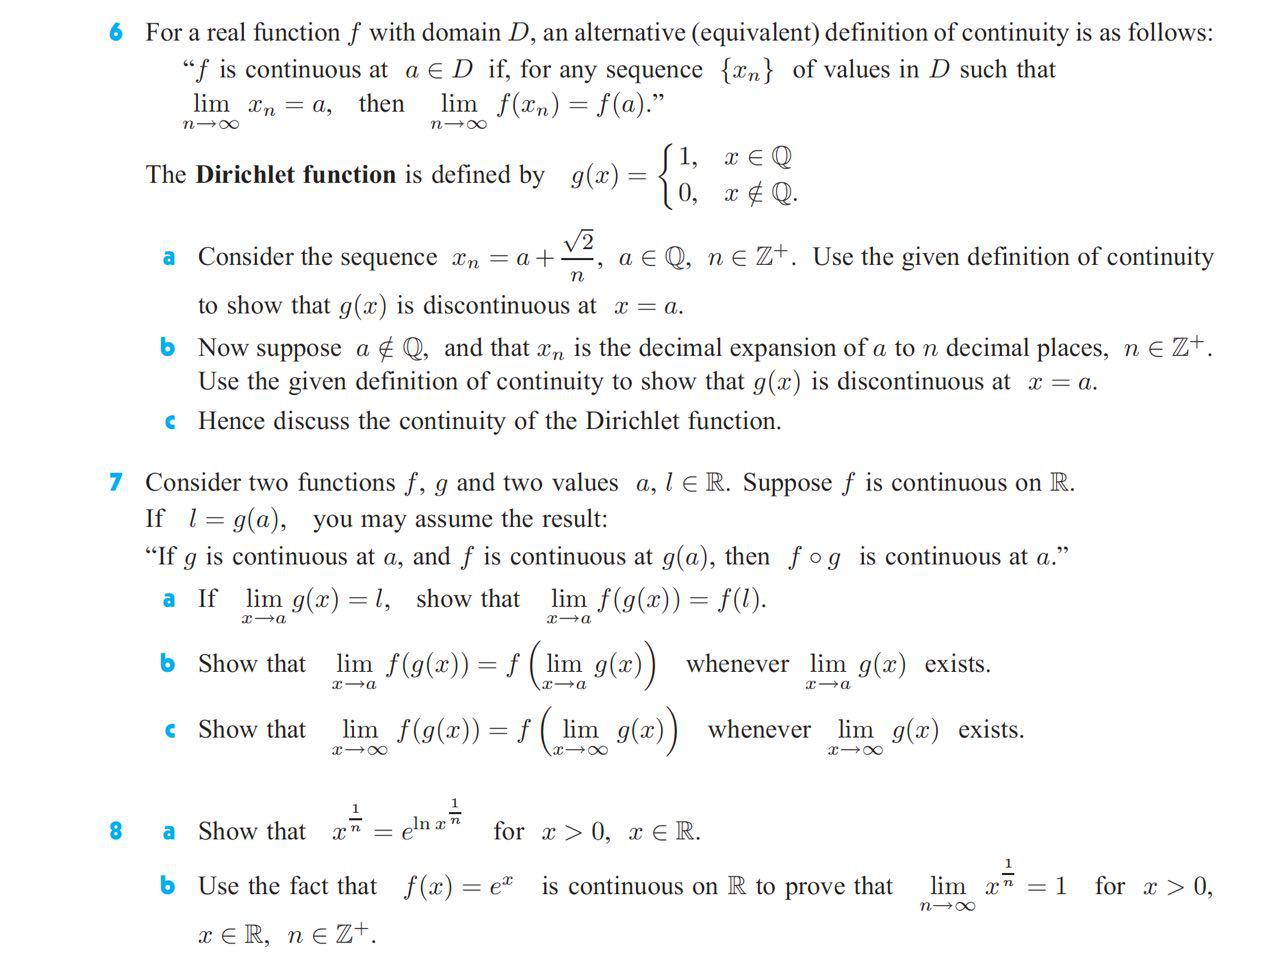
\includegraphics[width=0.95\linewidth]{photo_2019-06-01_00-00-41}
\end{center}

\newpage
\textbf{Hachette Aleph0 CDE Translation}
\begin{center}
\textbf{NEW PROGRAM}\\
Edition of May 14, 1971

\textbf{SECTION A}
\end{center}
OBLIGATORY SECTION

\textbf{Exponential and Logarithmic Functions}

\textbf{I.} Review of the notion related to continuity, limit, derivative, and real functions with one real variable. Derivative of composite functions.

One will admit without proof that if one numeric function is differentiable on an interval, and if its derivative is positive or zero on that interval, then it's growing in the broad sense on that interval, and that the image of a interval is an interval.

Geometric interpretation of the derivative.

Application on the study and the graphic representation of some simple functions (only on the numeric examples).

Function $x\mapsto x^n\,(n\in\mathbb{Z})$.

(One will not demand the candidates of baccalaureate to demonstrate directly the continuity of a function, nor to find directly a limit; one limit themselves only to utilize the general theorems and statements without proofs, and to talk about limits of sums, products, and quotients of functions).

\textbf{II.1.} Examples, taken from social and natural sciences, of functions whose increment on the whole interval $[x,x+l]$, for a given $l$, is proportional to the value of the function at the point $x$.

\textbf{2.} Study of sequences $n\mapsto f(n)$ such as $f(n+1)-f(n)=kf(n)$, $n\in\mathbb{N}$, calculation of $f(n)$, monotonicity of $f(n)$; limit of $f$ when $n$ tends to $+\infty$.

\textbf{3.} One will admit the existence, for all strictly positive real $a$, of a unique continuous and differentiable function $f_a$ defined on $\mathbb{R}$, such that for all tuple of real numbers $(x,y)$ one has $f_a(x+y)=f_a(x)f_a(y)$ and $f_a(1)=a$. Calculation of $f_a(x)$ for $x\in\mathbb{Z}$ and $x\in\mathbb{Q}$. (One can admit the existence of an n-th root for all positive real numbers and all positive integer $n$).\\
Calculation of $f_a'(x)$ according to $f'_a(0)$.\\
Notation $a^x$ (exponential function of base $a$), properties of the exponents: $(a^b)^c=a^{bc}$, $(ab)^c=a^cb^c$. The sign and monotonicity of $f_a$, the limit of $f_a$ pour $x$ tends to $\pm\infty$

\newpage
\textbf{Beijing LGBT Center Presentation - Algebraic Topology and its Application in Modern Algebra}

\textbf{Admitted Fact (Fundamental Group of Circle).} $$\pi_1(S^1)\simeq\mathbb{Z}$$

\textbf{Theorem (Fundamental Theorem of Algebra, Topological Approach).} Every non-constant polynomial with coefficient in $\mathbb{C}$ has a root in $\mathbb{C}$.
\begin{proof}
Without loss of generality we may assume that the polynomial we are dealing with is monic, i.e. it's of the form $$p(z)=z^n+a_1z^{n-1}+\cdots a_n.$$ Suppose this polynomial has no root in $\mathbb{C}$, then for each real $r\geq0$ we may define a loop $$f_{r}(s)=\frac{p\left(r e^{2 \pi i s}\right) / p(r)}{\left|p\left(r e^{2 \pi i s}\right) / p(r)\right|}$$ in the unit circle with basepoint $1$. As $r$ varies, $f_r(s)$ is a path homotopy of loops with basepoint $1$. Since $f_0$ is a trivial loop $s\mapsto1$ and $f_r$ are in the same class of the fundamental group, we deduce that this equivalent class $[f_r]\in\pi_1(S^1)$ is zero up to isomorphism. Now fix a large value $r$, bigger than $|a_1|+\cdots+|a_n|$ and bigger than $1$. Then for a $z$ such that $|z|=r$ we have \begin{align*}|z^n|=|z||z^{n-1}|&>(|a_1|+\cdots+|a_n|)|z^{n-1}|=|a_1||z^{n-1}|+\cdots+|a_n||z^{n-1}|\\&>|a_1z^{n-1}|+|a_2z^{n-2}|+\cdots+|a_n|\\&\geq|a_1z^{n-1}+a_2z^{n-2}+\cdots+a_n|.\end{align*} Define a new polynomial $$p_t(z)=z^n+t(a_1z^{n-1}+\cdots+a_n).$$ By the previous inequality $p_t(z)$ has no root on the circle $|z|=r$ for $0\leq t\leq 1$. Define $$g_t(s)=\frac{p_t\left(r e^{2 \pi i s}\right) / p_t(r)}{\left|p_t\left(r e^{2 \pi i s}\right) / p_t(r)\right|};$$ this is a homotopy from the loop $\omega_n(s)=e^{2\pi ins}$ to $f_r$. By the admitted fact, $\omega_n$ is $n$ up to isomorphism. Since we have shown that $[\omega_n]=[f_r]=0$ up to isomorphism, we may conclude $n=0$, and thus the polynomial is constant.
\end{proof}

\newpage
\textbf{Algebraic Topology}

\textbf{MIT 18.905 Fall 2016 Lecture 1} \textbf{Theorem 1.5.} Any boundary is a cycle; that is, $d^2=0$.
\begin{proof}
Let $\vec{t}=\langle t_0,\dots,t_{n-2}\rangle\in\Delta^{n-2}$, and $\displaystyle\sigma=\sum_{i=1}^ka_i\sigma_i$, then we have \begin{align*}d(d\sigma)(\vec{t})&=d\left(\sum_{i=1}^ka_i\sum_{j=0}^n(-1)^jd_j\sigma_i\right)(\vec{t})\\&=\left(\sum_{i=1}^ka_i\sum_{j=0}^n(-1)^jd(\sigma_i\circ d^j)\right)(\vec{t})\\&=\sum_{i=1}^ka_i\sum_{j=0}^n\sum_{r=0}^{n-1}(-1)^{j+r}\sigma_i\circ d^j\circ d^r(\vec{t})\\&=\sum_{i=1}^ka_i\left(\sum_{j=0}^n\sum_{r=0}^{j-1}(-1)^{j+r}\sigma_i\circ d^j\circ d^r(\vec{t})+\sum_{j'=0}^{n-1}\sum_{r'=j'}^{n-1}(-1)^{j'+r'}\sigma_i\circ d^{j'}\circ d^{r'}(\vec{t})+\sum_{j=n}^n\sum_{r=0}^{n-1}(-1)^{j+r}\sigma_i\circ d^j\circ d^r(\vec{t})\right)\\&=\sum_{i=1}^ka_i\left(\sum_{j=0}^n\sum_{r=0}^{j-1}(-1)^{j+r}\sigma_i\circ d^j\circ d^r(\vec{t})+\sum_{j'=0}^{n-1}\sum_{r'=j'}^{n-1}(-1)^{j'+r'}\sigma_i\circ d^{j'}\circ d^{r'}(\vec{t})\right).\end{align*} Now $$d^j\circ d^r(\vec{t})=\langle\dots,\underbrace{0}_{r},\dots,\underbrace{0}_{j},\dots\rangle\text{ for }0\leq r<j\leq n$$ and $$d^{j'}\circ d^{r'}(\vec{t})=\langle\dots,\underbrace{0}_{j},\dots,\underbrace{0}_{r+1},\dots\rangle\text{ for }0\leq j'\leq r'\leq n-1.$$ There clearly exists a bijection between the index pair $(j,r)$ and $(j',r')$, namely $j'=r$ and $r'=j-1$ with inverse $r=j'$ and $j=r'+1$, and for these pairs of index pairs, the value of $(-1)^{j+r}$ and $(-1)^{j'+r'}$ differs by a sign, as desired.
\end{proof}

\textbf{TIMS Lecture Algebraic Topology Lecture 2} For every topological space $X$, establish a group isomorphism $$\mathbb{Z}\pi_0(X)\simeq H_0(X,\mathbb{Z}),$$ where $\pi_0(-):(\mathbf{Top})\to(\mathbf{Grp})$ is the zeroth homotopy group functor, aka the path-connected component functor; $\mathbb{Z}[-]:(\mathbf{Set})\to(\mathbf{Ab})$ the free abelian group functor; and $H_0(-,\mathbb{Z}):(\mathbf{Top})\to(\mathbf{Ab})$ the zeroth homology group functor with integer coefficients.

\textbf{Solution.} First we proceed with the $\rightarrow$ direction. For each path-connected component $A\subset X$ we appeal to the axiom of choice and pick an arbitrary point $a\in A$. Observe that $a\in Z_0(X)=\ker\partial_0$ since the kernel of a constant zero map is its entire domain and that $a\notin B_0(X)=\operatorname{im}\partial_1$ since there are only two possibilities of boundary for a $1$-simplex: either $0$ if it is a cycle, or two distinct points with opposite signs, and none of the linear combinations of each can produce a singularity $+a$. Note that if the coefficient before $A$ is negative, then we will associate a $-a$ to it instead of a $+a$. This association extends via linearity: for $\sum_i\phi(A_i)A_i$, we pick $a_i\in A_i$ and associate $\sum_i\phi(A_i)a_i$ to it. Notice that this association is well-defined since for a change of picked point $a\in A$ to $a'\in A$ does not change the coset associated to it: let the original coset associated to it be $B=[+a]$, since $A$ is path-connected we can produce a $1$-simplex $\sigma$ with $\sigma\circ\iota_0=a'$ and $\sigma\circ\iota_1=a$, and its boundary will thus be $+a'-a$, and this, added to $B$, is exactly what we need---a representative of coset in $B$ that have a singularity $+a'$. It's trivial to check that this association, denoted $\chi$, is a group homomorphism. Now we proceed with the $\leftarrow$ direction. For each path-connected component $A$ and coset $B\in H_0(X)$, we reduce the coset to its canonical form by adding inverse $1$-simplexes to cancel the $(+,-)$ pairs, then we count the remaining points with sign as $k$ and associate $kA$ to $B$. It is also trivially verified that this, denoted $\psi$ is a group homomorphism, and that $\chi\circ\psi=\mathbb{1}$ and $\psi\circ\chi=\mathbb{1}$, and we have the desired isomorphism.\qed

$$
\begin{tikzcd}
A\arrow[r,"h"]\arrow[d,hook]&B\arrow[d,"i_1"]\arrow[ddr,bend left,"f_1"]\\C\arrow[r,"i_2"]\arrow[drr,bend right,"f_2"]&B\cup_hC\arrow[dr,dotted,"{\exists!f}"]\\&&Q
\end{tikzcd}
$$

$$
\begin{tikzcd}
X\arrow[r,"g_1"]\arrow[d,"g_2"]&X_1\arrow[d,"i_1"]\arrow[ddr,bend left,"f_1"]\\X_2\arrow[r,"i_2"]\arrow[drr,bend right,"f_2"]&\frac{X_{1} \oplus X_{2}}{\left\langle (g_{1}(x),-g_{2}(x))\, | \,x \in X\right\rangle}\arrow[dr,dotted,"{\exists!f}"]\\&&Q
\end{tikzcd}
$$
\begin{center}\textbf{Figure 4.} Pushout in $(\mathbf{Ab})$\end{center}

\textbf{Prism Operator.}
$$\prescript{n}{}{P}_{[v_0,\dots,v_n]}^{[w_0,\dots,w_n]}(\sigma)=\sum_{i=0}^n(-1)^{i} F\circ(\sigma \times \mathbb{1}) |_{\left[v_{0}, \dots, v_{i}, w_{i}, \dots, w_{n}\right]}$$

$$\begin{tikzcd}
                 & 0 \arrow[d, hook]                                                     & 0 \arrow[d, hook]                                         & 0 \arrow[d, hook]                                 &        \\
\cdots \arrow[r] & A_{n+1} \arrow[d, "f_{n+1}", hook] \arrow[r, "\partial_{n+1}^A"]      & A_n \arrow[d, "f_n", hook] \arrow[r, "\partial_n^A"]      & A_{n-1} \arrow[r] \arrow[d, "f_{n-1}", hook]      & \cdots \\
\cdots \arrow[r] & B_{n+1} \arrow[d, "g_{n+1}", two heads] \arrow[r, "\partial_{n+1}^B"] & B_n \arrow[d, "g_n", two heads] \arrow[r, "\partial_n^B"] & B_{n-1} \arrow[r] \arrow[d, "g_{n-1}", two heads] & \cdots \\
\cdots \arrow[r] & C_{n+1} \arrow[d, two heads] \arrow[r, "\partial_{n+1}^C"]            & C_n \arrow[d, two heads] \arrow[r, "\partial_n^C"]        & C_{n-1} \arrow[r] \arrow[d, two heads]            & \cdots \\
                 & 0                                                                     & 0                                                         & 0                                                 &       
\end{tikzcd}$$

\newpage
AP Calc $\to$ Baby Rudin - (Compactness and Connectedness, EVT, IVT, UCT, \textbf{Topological properties of the space is the most general intrinsic properties thereof}), Inverse Function Theorem (Hadamard, \textbf{topological properties of the map extends local property to global property}), Implicit Function Theorem (Differential Equation)

Baby Rudin (Munkres) $\to$ Tu Manifold - de Rham Cohomology (cohomologouity of form, counterexample of closed form being exact, \textbf{de Rham cohomology group reveals the topological nature of manifold as a space, e.g.} $H_{\mathrm{dR}}^{0}(M) \cong \mathbb{R}^{m}$), Regular Level Set Theorem (Brouwer's Fixed Point Theorem)

Brouwer (Fundamental Group and Homotopy Group) \& de Rham Cohomology (try to find similar construct) $\to$ Hatcher algebraic topology: triangularization of space/CW-complex (simplicial homology, cellular homology), once again \textbf{topological nature of space captured by algebraic structure}: $\mathbb{Z} \pi_{0}(X) \simeq H_{0}(X, \mathbb{Z})$, $\pi_1(X,x_0)\simeq H_1(X,\mathbb{Z})$, project: cellular approximation theorem (current), project: computational homology (current)

\noindent\makebox[\linewidth]{\rule{\paperwidth}{0.4pt}}

Let me tell you a story of a math girl, a cyclic story of interest, exploration, frustration, satisfaction, and most importantly knowledge acquisition and contribution, a story of her following her intellectual antecedents experiencing the methodologies by which we human explored the world and its disciplines, a story of her and her first love, a story of her and mathematics, a story of me.

``For any epsilon greater than zero, there exists a delta greater than zero, such that...," then my journey begins with Rudin's \textit{Principles of Mathematical Analysis}. Even today, highlights of mathematical analysis still triggers my memory (and some of them also apply to me current study). I remember when I was introduced to topology induced by metric; compactness and connectedness, EVT and IVT and and UCT; what I learned in AP Calculus is brought to me again but with rigorous language. I remember the inverse function theorem from Rudin and the theorem of Hadamard, the global version; "certain topological properties of spaces and maps extends local property to global property," like they say. There are three things I feel unsatisfactory about Rudin: topology, differential geometry, and measure theory, each occupying a chapter\footnote{2, 10, and 11; though it's an analysis book so it's extenuating}. For those, I turned to Munkres \textit{Topology}, Tu \textit{Introduction to Manifolds} and Lee \textit{Introduction to Smooth Manifolds}, and Stein \textit{Real Analysis}. 

If there's a most important take away from Tu, I would say it's de Rham cohomology (which makes me unusual since most people love Stokes' theorem more than de Rham theory, probably because I'm the more theoretical type), which paves a road for me to what I'm currently studying, homological algebra and algebraic topology. de Rham cohomology is the first construct with $\frac{\ker}{\operatorname{im}}$ liked form I ever encountered which captures the element in the kernel that is not in the image. This construct for chain/cochain complex is useful when it is used to reflect the nature of a topological space: such as $n$-simplex with boundary map in singular homology and that $\mathbb{Z}\pi_0(X,x_0)\simeq H_0(X,\emptyset;\mathbb{Z})$\footnote{and more general, Hurewicz theorem} or $n$-form in exterior derivative in de Rham cohomology and that $H^0_{\mathrm{dR}}(M)\simeq\mathbb{R}^m$. At the time, I was so intrigued by the multilinear algebra of differential forms and cohomology, but tired of tedious coordinate related calculations (in which I always make mistakes), then I found a lecture note on algebraic topology, which brings me the similar idea, but without coordinate-related calculations.

I proved the zig-zag lemma for homology defined for chain complex. It generates a long exact sequence for any short exact sequence of chain map. A technique called diagram chasing is used: I wish to find a $a\in A_{n-1}$ for a specific $c\in C_n$ given, like shown in the following diagram. I observe that since $0$ the trivial module is the starting and ending point of the short exact sequence, so that from the exactness of map $\ker=\operatorname{im}$ the first map in the sequence is injective, and the second is surjective. So we can ``chase" the element one step up to an element $b'\in B_n\setminus\ker\partial_n^B$. By assumption $c\in\ker\partial_n^C$, we have $(g_{n-1}\circ\partial_n^B)(b)=0=(\partial_n^C\circ g_n)(b)$ and this allowed me to chase on step up to an element $a\in A_{n-1}$. Recall that I used a choice of preimage of a surjective (but possibly not injective) map. The next step requires me to prove that the value of this correspondence $\partial$ does not depend on that choice but only the parameter $c$. Another useful note in this argument is that there is functor $H_*(-):(\mathbf{Top}^2)\to(\mathbf{Gr}_{\mathbb{Z}}^+)$ such allows me to apply this result of homological algebra to algebraic topology.

Besides things mathematical, I'm very well acquainted, too, with matters about computer science.

\newpage
Let me tell you a story of a math girl, a cyclic story of interest, exploration, frustration, satisfaction, and most importantly knowledge acquisition and contribution, a story of her following her intellectual antecedents experiencing the methodologies by which we human explored the world and its disciplines, a story of her and her first love, a story of her and mathematics, a story of me.

The first insight worth sharing to me is the distinct 

I believe what makes homology theory and algebraic topology intriguing to me is that the central notions of the subject, homology and cohomology of various chain complexes characterizing topological spaces (e.g. singular chain complex, CW complex, etc.) is, philosophically speaking, one of the most fundamental topological invariant of those spaces; though they might be difficult to be understood intuitively, for example in torsion-free spaces, singular homology captures the higher-dimensional analogy of ``holes" of topological space, when considered in an ambient Euclidean space (this intuition actually works for an unexpectedly wide range of spaces since every compact metrizable space of Lebesgue covering dimension $m$ can be imbedded in a Euclidean ambient space of dimension $2m+1$), or even lack intuitive meaning in some spaces (e.g. torsionful spaces).

\noindent\makebox[\linewidth]{\rule{\paperwidth}{0.4pt}}

``You have a solid foundation in mathematical analysis," so exclaimed Prof. Yitang Zhang. That was the first time I am accredited by a professional in the field of mathematics. ``You are like a second year undergraduate, though you're only 15," he said, when he watched me doing an rather not-so-trivial exercise in Rudin's \textit{Principles of Mathematical Analysis} (the integral of the Thomae function) and read my note collection on mathematical analysis.

\noindent\makebox[\linewidth]{\rule{\paperwidth}{0.4pt}}

One day, an Olympiad problem was brought to me by a fellow student; it requires me to find the shortest path between two points in a plane with an circular area obstructed. The solution comes immediately from the problem settings: two tangent lines segments and an arc of the circle would suffice. But then I started wondering how a proof can be constructed and what if the problem is given in a more general setting, say 

\noindent\makebox[\linewidth]{\rule{\paperwidth}{0.4pt}}

\begin{enumerate}
\item Yitang Zhang accredited me;
\item Read AP Calculus in grade 7;
\item Able to use {\LaTeX} since grade 8;
\item Grade 9 - Haskell; TAPL@PKU
\item French - 2018;
\item analysis, algebra - 2016-2017
\item DG - 2018;
\item AT - 2019;
\item Tutoring
\end{enumerate}

\newpage
My journey of mathematics started in 2014. Like any young and curious little girl, I received a present, an AP Calculus textbook, from a dear teacher. Its obscure content on the notion of limit made my learning unsatisfactory. I'm unable to accept the notion of ``arbitrary closeness". Then I tried to use my language to fill the emptiness of it. First I was convinced that I have to find a way to achieve ``infinitesimal". For that I defined a special kind of ``list" of numbers, progressing becoming less than any number ``nominable". And any function whose values form a difference between a number $l$ and elements of such a list with another such list plus an $x_0$ as parameters would be considered to have a ``limit" $l$ at point $x_0$. This was found out later by a math teacher to be ``surprisingly similar to the definition of limit given by Cauchy in his \textit{Cours d'Analyse}."

Recently I'm also into the theories of pre-tertiary mathematical education. I believe that the idea of general education of modern mathematical notions is crucial in current and future secondary mathematical education. To verify that, I conducted a social experiment. I gathered a group of A-Level students who are applying for math-related majors, then, several other teachers and I started to teach an alternative curriculum, in which modern notions are incorporated with the classical content. For example, when we were teaching the properties of the real line, the notion of topological space and ordered field were introduced; when we were teaching the exponential and logarithm functions, the properties of general sequence and series of functions were given. Theorems that requires higher knowledge to deduce or are too technical to be presented at the pre-tertiary phase, such as the equivalent definitions of the real number, was admitted without proof. This experiment is still on-going and the assessment of the result will be drawn from the comparison of our students against others trained in the traditional way, in the aspect like acceptance, MAT score, interview feedback, and GPA performance. After careful reading of related researches and historic literature, I found out that my approach is surprisingly similar to that of Bourbaki, and I did learn from the failure thereof and refined my current approach. I would say this experiment enhanced my understanding of the relation between education and society, provoked my interests in mathematics and teaching further, and gave me new insights of the subject I love, and I would say that this experiment and research will continue.

Besides studying and researching on my own, I also love sharing knowledge. In 2017, I organized a mathematical history seminar on the general use of analytic methods in the history of mathematics. My lecture topic is calculus of variation, with application to the brachistochrone problem and the isoperimetric problem, among others, which includes topics like the fundamental theorem of algebra, the Jordan curve theorem, the Sard's theorem, the Brouwer's fixed point theorem, etc. As an organizer, I talked to my high school's coordinator for booking the classroom for the seminar, designed and opened up webpage for paper submission and audience registration, prepared the projector and computer, set up the posters and made address to the students about the seminar on our school's assembly; also as a lecturer, I prepared the lecture note and the slides, all exquisitely typeset with {\LaTeX}, overcame my social anxiety and voice dysphoria, and on the seminar day answered every question with detailed argument and patience.

As for my recent study, I am currently working on homological algebra and commutative algebra, and, consequently their application in algebraic topology and algebraic geometry. I'm following Davis \& Kirk's \textit{Lectures in Algebraic Topology} and the open-sourced textbook \textit{The Stacks Project}. With the help of a Ph.D. student from PKU (Peking University), I will have a chance to audit courses on homology theory and commutative algebra in PKU in the first semester of 2019-2020 academic year. Preparing myself with sufficient background in algebra and topology, I see this great opportunity more valuable than ever. Though it's probably too early to say, I look forward to a mathematical career in topology and geometry, which is the main reason I've started so early in self-studying mathematics especially modern notions such as commutative algebra and category theory. I see my tertiary and higher education as a new opportunity of closer integration of resources and opportunities of application of my knowledge, as well as a platform to develop it further. For that, as a mathematical student, I request you to consider me for the admission into the undergraduate department of mathematics in the 2020-2021 academic year.

\newpage
``I'm a girl, a girl who is born inside a boy's body, and it's not my fault," I finished my speech in the TA (transgender anonymous) session in Beijing LGBT Center. It is something I would never imagine two years ago: confidence and extraordinariness, in a way that allows me to give a speech, as a female, about my identity, for the community.

Like most of transgenders, I discovered my identity so early in life that I even can't remember when exactly it is. And it isn't me until puberty, when I started to feel the damage of gender dysphoria, a person who is self-enclosed, socially anxious, underconfident, and depressed, like me 2 years ago. Since then, I became less proactive in socializing scenarios, lost friends, got unsatisfactory grades. I found myself less and less confident in daily life, avoiding going to restrooms and change rooms, trying to be the same as other cisgender boys and hide my identity, for example.

But this all changed in 2018, when I finally nerved myself to come out with my parents. With help from my gender therapist, they understood my identity and decided to give support. Then I started my transition: trying clothes that are female oriented, experimenting with cosmetics, etc. But I would say now the most important part is my voice training. In China, not so many people know and really understand transgenderism, and they tend to apply implicit violence upon us like verbal harassment and humiliation, and this hurt my confidence multiple times. Once I was in a cosmetics store with a cisfemale friend. I was talking to her and the staff clearly heard my voice and said to me: ``that boy, please move to this side, you're blocking the light," as if my friend is the only customer he cares about, and as if I'm my appearance isn't passing enough to let him use the proper pronoun. I ran away and decided I would work so hard on my voice so that no one can deny my identity anymore. Indeed, it was difficult, possible due to my unorthodox training method. My vocal cord hurt on an hourly basis. But eventually I overcame the obstructions and achieved a relatively satisfactory result.

Since then, my appearance and voice became consistent. I would finally be able to speak to the crowd. I went back to that cosmetics store and found the same staff. This time he genuinely introduced me to their products and referred to me a beautiful lady. That did strengthen my confidence: in the past, when I organized my mathematical seminar, I was nervous about my voice, but now I stand up confidently, ask, answer questions and interact with the lecturer when auditing courses in PKU (Peking University). I also studied more theories on transgenderism and gender, which brings the speech aforementioned possible. I now live full-time as a female, enjoying socializing both in the real world and online, with voice and video, proudly showing my image to the world, and having made new friends. My transition shaped me, letting me become the woman I am now, and my identity as a female gave me insights about myself, gender, love, and the world, like a second puberty, except for this time it's a happy one, and is an important part of me and my journey of life.

\begin{tabularx}{\linewidth}{c|X}
\thead{Activity}&\thead{Description}\\\hline
Types and Programming Languages&Audited a course TaPL in PKU about theoretical computer science; got 85/100 on the exam\\\hline
Calculus Book&Attempted to write a rigorous calculus note series for my classmates\\\hline
Voluntary Service Translation&Translated for Beijing LGBT Center transgender related sessions\\\hline
Literature Review&Wrote a literature review on the interdiscipline research of transgender and HIV prevention for Beijing LGBT Center\\\hline
IMMC 2018&Participated in the International Mathematical Modeling Challenge 2018; got finalist award\\\hline
Contribution to Wuli.wiki&Contribution to a Chinese online physics wiki project; the topic contributed is differential geometry and general relativity.\\\hline
Book Project - algebra-for-cute-girls&Authored a self-contained book, using categorical language to formulate algebra.\\\hline
Book Project - elementary-analysis&Authored a self-contained book to help high schoolers get familiar with prerequisite of analysis and modern mathematics; Main content: first-order logic, natural deduction, ZFC axiomatic set theory, number systems
\end{tabularx}

\newpage
I love community work and collaboration in my academic work. Moreover, I'm actually an open source projects leader. I have 2 open source textbook project, algebra-for-cute-girls, which is a graduate text aiming to formula relatively self-contained contents on algebra using categorical and higher categorical language, and elementary-analysis which is an attempt to help mathematical students transition from high school to university by providing them the mathematical foundations to modern analysis and other branches, such as first-order logic, natural deduction, ZFC axiomatic set theory, construction of number systems, etc. I also contribute to another open source wiki project, wuli.wiki, which provides self-contained physics content for high school and undergraduate students, much like the stacks project by Columbia University.

In the process of creating and contributing to these projects, I applied academic skills as well as interpersonal collaboration skills. I helped my co-authors with technical problems like using {\LaTeX} and GitHub. We used peer-reviewing process to ensure the validity and quality of our drafts. I, specifically, as a leader, must know when to brainstorm and come up with ideas with my co-authors, but also when to make the tough decisions like which parts of the book stay and which part go. From past events I acquire the faith habitually that I am not suitable to be a leader or decision maker. But in these practices I developed these skills and become a relatively successful leader.

\newpage
Few days ago, I read a message: graduate school of science of Hiroshima University posted a tenure-track oriented offer for a position of associate professor that is specifically exclusive for female applicants. To me, this ringed a bell. The intention of such offers, should it exist, is undoubtedly of goodwill, the consideration of promoting females’ participation and engagement in the field of science, but it is crucial for us to understand, in the context of society and academia, if this is a well-considered action.

There are a few pending questions to be discussed. First, will this work?  In Japan, the numerical distinction of the male versus female doctoral application and graduation rate is significant, not to mention the low chance of female academicians entering research positions. The impact of similar policy may not be as effective as we originally predict, since it doesn’t solve the fundamental issue that Japanese culture and society implicitly discourage females in participating those disciplines that are considered male dominant. Second, is this gender discrimination? I suppose so; the definition of gender discrimination is the distinctive treatment toward genders, and surely providing a special offer for females falls in to that category. It triggers my thoughts on the question: if we’re unable to change the societal situations at once, is it acceptable to incline toward the weak group in the selection process temporarily? This has been done worldwide; and I believe the university I’m applying is also enforcing the policies, out of good intention, inclined toward minorities. Maybe in the future I would have grounds for a definitive answer, but for now I can only pose this question; I do not know how to judge a moral situation like this.

Another question I would pose, in my position, is that, how do I prove that I am competitive enough for my offer? The policies inclines toward me and similar minorities. What can we do as females, transgenders, Asians, etc. to prove that we are not accepted for our minority status but for our endurance and accomplishments? Remember the Republican candidate Ben Carson; he is black, and thus being inclined toward by the law, but at his position, this not only does not support him, but gives him another burden: he has to prove that he is worth of choice because of his talent and dedication, not because of he being black. In the future, I would face the similar situations when competing with my fellows. What should I do to change this situation? I wish in the future I would have the answer for that.

\newpage
Thursday, February 28, 2019 is a special day, the day when the 10 campus system of University of California discontinued the renewal of its subscription with the world's largest academic publisher, Elsevier. This day marks a hard-fought victory of the academic community with the idea of openness I believe in.

When I was young, there was this girl who knows, to me at that time, everything and who I yearn for in my primary years. I yearn for her knowledge of advanced mathematics such as exponentials and logarithms, for her ability to communicate in English and Cantonese with the foreigners fluently, for her unique interpretation of ancient Chinese corpuses. I wondered how she can be so excellent and wanted to be like her. It turns out that her parents are both Ph.D. and value her education so much that even pay for her to exchange abroad. This notified me, in the early days of my life, the significant role in acquiring them one's background and resources play: If you have highly educated parents, a lot of money, and a good geographic community then you can have knowledge which will make you again be highly educated, rich, and in a good community, and most importantly, make you powerful. But if you're without them, at least in China, there will be an opposite circle waiting for you.

And this is why I support the most radical ideas in the open academic community: I have dream that one day no one should ever pay for education and acquiring knowledge. I support the community with my ideas with action since when I started publishing, outputting, and creating. For example, I am publishing every snippet of \LaTeX code I wrote (typically about mathematics) online with license allowing anyone to read, modify, and republish. I petitioned for GitHub to which I publish my Julia and Mathematica codes not being acquired by Microsoft, although it turns out that it doesn't work. I donated to and spreaded Wikipedia, SciHub, LibGen and other sites that supports my idea. I sincerely hope that one day my dream of free and open knowledge access will come true.

\newpage
Everyone, such as I, loves romance. Internet give us the opportunity to pursue romance and intimate relationships online, but this journey is relatively undesirable to some of us: to be specific, I am talking about the sexual minorities in China.

There are social network apps for dating in China, of course; in fact, plenty of them with a diversity of functions like voice/"soul" matching, random chatting, public surveying, etc. But they at most times gives me and other minority people in China negative experiences. For example, I matched a person on an app called Douli. For a bit of background this app allows its user to set their SOGIE (sexual orientation - gender identity, expression), which is pretty great at the first glance to me and I set my real SOGIE. But when this person heard my voice and saw my SOGIE, he constantly negate my identity and claims that I am a male pervert. This really hurt me and made me uninstall this app at once.

This bad experience also inspired me in a way that motivates my friends at Beijing LGBT Center and me to come up the idea of writing an real minority-friendly dating app of our own. We did this from scratch: planned for SOGIE education functions like videos and in-app tests, contacted friendly organizations for spreading the app, etc. (TODO write a closure)

\newpage
\begin{enumerate}[label=\arabic*.]
\item $5\pi\,m^2/m$, i.e. $5\pi\,m$;
\item $f(x)=-\cos x+3$;
\item $2\text{ in}\times 2\text{ in}$;
\item $3$;
\item $-\ln\circ\cos$, whose domain is $\mathbb{C}\setminus\{n\pi\,|\,n\in\mathbb{Z}\}$;
\item $\displaystyle\frac{125}{6}$;
\item $9\pi$;
\item $\displaystyle\frac{\pi}{32}$;
\item $\displaystyle\frac{\sqrt{5}}{3}$, $\displaystyle\frac{2}{\sqrt{5}}$, $\displaystyle\frac{3\sqrt{5}}{5}$, $\displaystyle\frac{3}{2}$;
\item $\displaystyle\frac{\sqrt{9+x^2}}{3}$;
\item $7$;
\item $\displaystyle y(x)=C_1x^{-2}+C_2 x$;
\item $\displaystyle y(x)=\frac{1}{2}e^{3x}x^2+C_1e^{3x}+C_2e^{3x}x$;
\item $\displaystyle-\frac{h(1+r)}{r-1}$;
\item This Question is missing;
\item $10\sqrt{2}$;
\item $-7$;
\item $xy\cos xy+\sin xy$;
\item $\displaystyle\frac{7}{12}$;
\item $\displaystyle\frac{1}{8}$.
\end{enumerate}

\textbf{Theorem.} Let $f:I\to\mathbb{R}$, that $\lim_{x\to a}f(x)=L$, and that $\lim_{x\to a}f(x)=R$, then $L=R$.
\begin{proof}
Proceed by proof by contradiction. Without loss of generality, set $L<R$. Then by definition, we have that for all $\varepsilon>0$, there exists $\delta_1>0$ such that for any $x_1$ with $|x_1-a|<\delta_1$, $|f(x_1)-L|<\varepsilon$, and for the same $\varepsilon$, that there exists $\delta_2>0$ such that for any $x_2$ with $|x_2-a|<\delta_2$, $|f(x_2)-R|<\varepsilon$. Take $\varepsilon=\frac{R-L}{2}$, then the above implies that for $x$ with $|x-a|<\min\{\delta_1,\delta_2\}$, $|f(x)-L|=f(x)-L<\frac{R-L}{2}$, i.e. $f(x)<\frac{R+L}{2}$; by the same manner, we can also deduce $f(x)>\frac{R+L}{2}$, thus a contradiction.
\end{proof}

\newpage
{\Huge Homotopy Invariance of de Rham Cohomology}

\textbf{Theorem (Cartan's Magic Formula).}

\textbf{Theorem (Whitney's Approximation Theorem).}

\end{CJK*}
\end{document}